


\frame{
Three planes form the boundary of a solid in the first octant\footnote{成$45$度视角的位置,八分圆}, which is shown in the following figure. 
\begin{figure}
\begin{center}
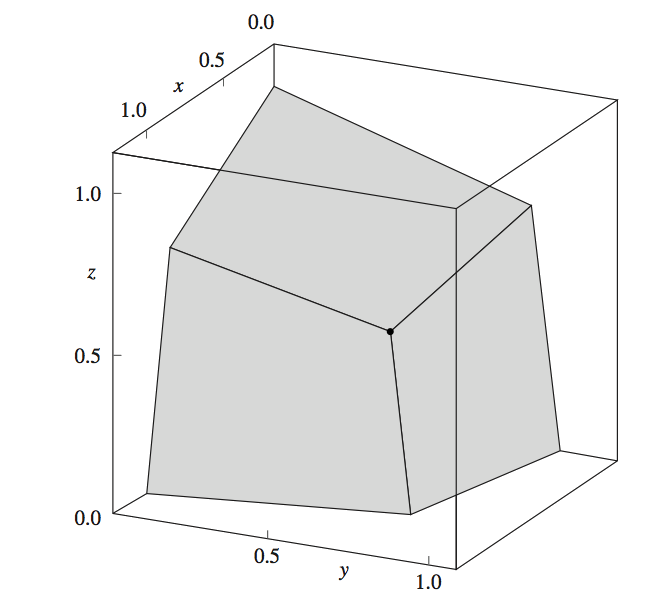
\includegraphics[width=45mm]{chap-2/fig_3-1.png}
%\caption{The portion of a sphere of radius $r$ that is to be submerged to a depth $d$}
\end{center}
\end{figure}
Suppose that the equations for these planes are
\begin{equation*}
\begin{array}{r r r r}
5x + & y + & z = & 5 \\
x + & 4y + & z = & 4 \\
x + & y + & 3z = & 3
\end{array}
\end{equation*}
}

\frame{
\begin{block}{}
{\Large What are the coordinates of the point of intersection of the three planes? }
\end{block}
\begin{center}
$\Downarrow$
\end{center}
{\Large Gaussian elimination} can be used to find the solution of the linear system
\begin{center}
$\Downarrow$
\end{center}
\begin{equation*}
\begin{array}{ l l }
x & = 0.76 \\
y & = 0.68 \\
z & = 0.52
\end{array}
\end{equation*}
}


